% Options for packages loaded elsewhere
\PassOptionsToPackage{unicode}{hyperref}
\PassOptionsToPackage{hyphens}{url}
%
\documentclass[
]{article}
\usepackage{lmodern}
\usepackage{amssymb,amsmath}
\usepackage{ifxetex,ifluatex}
\ifnum 0\ifxetex 1\fi\ifluatex 1\fi=0 % if pdftex
  \usepackage[T1]{fontenc}
  \usepackage[utf8]{inputenc}
  \usepackage{textcomp} % provide euro and other symbols
\else % if luatex or xetex
  \usepackage{unicode-math}
  \defaultfontfeatures{Scale=MatchLowercase}
  \defaultfontfeatures[\rmfamily]{Ligatures=TeX,Scale=1}
\fi
% Use upquote if available, for straight quotes in verbatim environments
\IfFileExists{upquote.sty}{\usepackage{upquote}}{}
\IfFileExists{microtype.sty}{% use microtype if available
  \usepackage[]{microtype}
  \UseMicrotypeSet[protrusion]{basicmath} % disable protrusion for tt fonts
}{}
\makeatletter
\@ifundefined{KOMAClassName}{% if non-KOMA class
  \IfFileExists{parskip.sty}{%
    \usepackage{parskip}
  }{% else
    \setlength{\parindent}{0pt}
    \setlength{\parskip}{6pt plus 2pt minus 1pt}}
}{% if KOMA class
  \KOMAoptions{parskip=half}}
\makeatother
\usepackage{xcolor}
\IfFileExists{xurl.sty}{\usepackage{xurl}}{} % add URL line breaks if available
\IfFileExists{bookmark.sty}{\usepackage{bookmark}}{\usepackage{hyperref}}
\hypersetup{
  pdftitle={The Price of Police},
  pdfauthor={Robert Crump},
  hidelinks,
  pdfcreator={LaTeX via pandoc}}
\urlstyle{same} % disable monospaced font for URLs
\usepackage[margin=1in]{geometry}
\usepackage{longtable,booktabs}
% Correct order of tables after \paragraph or \subparagraph
\usepackage{etoolbox}
\makeatletter
\patchcmd\longtable{\par}{\if@noskipsec\mbox{}\fi\par}{}{}
\makeatother
% Allow footnotes in longtable head/foot
\IfFileExists{footnotehyper.sty}{\usepackage{footnotehyper}}{\usepackage{footnote}}
\makesavenoteenv{longtable}
\usepackage{graphicx,grffile}
\makeatletter
\def\maxwidth{\ifdim\Gin@nat@width>\linewidth\linewidth\else\Gin@nat@width\fi}
\def\maxheight{\ifdim\Gin@nat@height>\textheight\textheight\else\Gin@nat@height\fi}
\makeatother
% Scale images if necessary, so that they will not overflow the page
% margins by default, and it is still possible to overwrite the defaults
% using explicit options in \includegraphics[width, height, ...]{}
\setkeys{Gin}{width=\maxwidth,height=\maxheight,keepaspectratio}
% Set default figure placement to htbp
\makeatletter
\def\fps@figure{htbp}
\makeatother
\setlength{\emergencystretch}{3em} % prevent overfull lines
\providecommand{\tightlist}{%
  \setlength{\itemsep}{0pt}\setlength{\parskip}{0pt}}
\setcounter{secnumdepth}{-\maxdimen} % remove section numbering
\usepackage{indentfirst}
\usepackage{booktabs}
\usepackage{longtable}
\usepackage{array}
\usepackage{multirow}
\usepackage{wrapfig}
\usepackage{float}
\usepackage{colortbl}
\usepackage{pdflscape}
\usepackage{tabu}
\usepackage{threeparttable}
\usepackage{threeparttablex}
\usepackage[normalem]{ulem}
\usepackage{makecell}
\usepackage{xcolor}

\title{The Price of Police}
\author{Robert Crump}
\date{9/5/2021}

\begin{document}
\maketitle

\hypertarget{introduction}{%
\section{Introduction}\label{introduction}}

\setlength{\parindent}{5ex}

2020 was a year like no other that compelled many Americans to
fundamentally reconsider how their cities are policed. In Chicago, this
reckoning came to a head during a weekend of protests and looting after
a Minneapolis police officer murdered George Floyd on May 25th.
Chicago's mayor, Lori Lightfoot, enacted emergency powers that
effectively shut down the central city while Chicago Police Department
(CPD) officers fanned out through the city to quell the unrest. The
city's iconic river-spanning bridges were raised, interstate ramps were
blockaded, the Chicago Transit Authority temporarily suspended service,
and the Governor deployed the Illinois National Guard to deter further
violence. The Summer of 2020 saw unfolding reprisals of civil unrest in
different parts of the city \footnote{\url{https://www.chicagotribune.com/news/breaking/ct-cb-george-floyd-fallout-impact-chicago-20201006-lkndggmch5emjiefplywhcaeou-story.html}}
that persisted into the Fall. As the dust settled in Chicago and
elsewhere, people across the country grappled less with the ``why'' and
more with the ``how'' of police reform. Police department budgets
received new levels of scrutiny as many citizens and politicians openly
advocated and mobilized for sweeping change. \setlength{\parindent}{5ex}
The future of local policing depends largely on how municipal
governments choose to allocate resources. Reimagining public safety and
charting a new path that hopefully leads cities and the nation away from
our troubled past requires a clear-eyed view of where we currently
stand. The City of Chicago maintains a large Open Data Portal that
contains City Budget Ordinances going back to 2011. This report examines
the Fiscal Year 2021 Budget Ordinance with particular focus on the CPD
budget and related appropriations. The goal of this report is to be
strictly descriptive while providing a base level of knowledge for other
researchers and curious citizens. However, it's worth noting that the
choice of what to measure and how to present data is inherently
subjective. \setlength{\parindent}{5ex} Summer 2021 has been a busy
season for Chicago's City Council, particularly regarding the CPD. In
July, the City Council threatened a vote of no confidence in the CPD
Superintendent appointed by the Mayor unless he agreed to a public
grilling on community violence \footnote{\url{https://chicago.suntimes.com/city-hall/2021/6/30/22557658/chicago-violence-shootings-fourth-july-weekend-police-plans-brown-council-aldermen-special-meeting}}.
Weeks later, the same Council passed the Mayor's proposal for a citizen
oversight board that she originally crafted as the President of the
Police Board \footnote{\url{https://blockclubchicago.org/2021/07/21/city-council-approves-first-ever-civilian-led-commission-to-oversee-chicago-police-department/}}.
The recently negotiated contract between the City and the Fraternal
Order of Police (CPD union) will substantially increase the CPD budget
while also adopting new accountability measures recommended by the
Department of Justice \footnote{\url{https://news.wttw.com/2021/07/26/police-officers-get-back-pay-face-new-accountability-rules-under-proposed-8-year-deal}}.
On July 30th, the Civilian Office of Police Account ability began
searching for a new Chief Administrator \footnote{\url{https://www.chicagocopa.org/press/the-city-of-chicago-begins-official-search-and-selection-process-for-the-next-chief-administrator-of-copa/}}.
Police spending in Chicago is certain to go up over the coming years,
and how that money is spent will remain a contentiously argued topic.
\setlength{\parindent}{5ex} What may come of these new changes is hard
to predict for the beleaguered Department, and for the City. A shared
understanding of facts is the first step towards meaningful change, and
finding a path forward, at the very least, requires a compass and a map.
I used two sources for this initial report, both from the City of
Chicago Open Data Portal. The primary resource is the Fiscal Year 2021
Budget Ordinance \footnote{\url{https://data.cityofchicago.org/Administration-Finance/Budget-2021-Budget-Ordinance-Appropriations/6tbx-h7y2}},
and the secondary resource is the Fiscal Year 2021 Budget Ordinance --
Positions and Salaries \footnote{\url{https://data.cityofchicago.org/Administration-Finance/Budget-2021-Budget-Ordinance-Positions-and-Salarie/gcwx-xm5a}}
which is a detailed subset of the full budget ordinance.

\hypertarget{chicago-city-2021-budget-overview}{%
\section{Chicago City 2021 Budget
Overview}\label{chicago-city-2021-budget-overview}}

\setlength{\parindent}{5ex}

The City of Chicago, like most local governments in the United States,
divides its budget into three broad categories: the general fund,
enterprise funds, and special revenue funds. The City of Chicago calls
its general fund the Corporate Fund, which contains most of the CPD
budget. Enterprise and special revenue funds are highly restricted in
discretionary spending choices because they require stability to support
essential services. The largest enterprise fund for most US
municipalities is the water and/or sewer funds. Special revenue funds,
such as fiduciary funds (pensions), are also legally structured to
resist changes in spending choices between election cycles. Although
municipal general funds permit more flexibility, most of the budget is
similarly constrained under contract, such as, for example, the Chicago
FOP contract. The motivating goal of constrained budgeting is stability
and predictability of public investment. Moreover, the dynamics of
political economy compels negotiators to demand credible commitments
from politicians who may or may not be in office for the duration of a
contract. \setlength{\parindent}{5ex} When engaging with something like
the City of Chicago budget, the first noticeable characteristics are its
size and complexity. Through close study and data manipulation using R,
I've attempted to display these characteristics while illustrating my
decisions for the sake of interpretation and gathering insight by
narrowing focus on particular datapoints. To start, let's get a picture
of the proportions of every named City fund using a treemap chart.

\begin{center}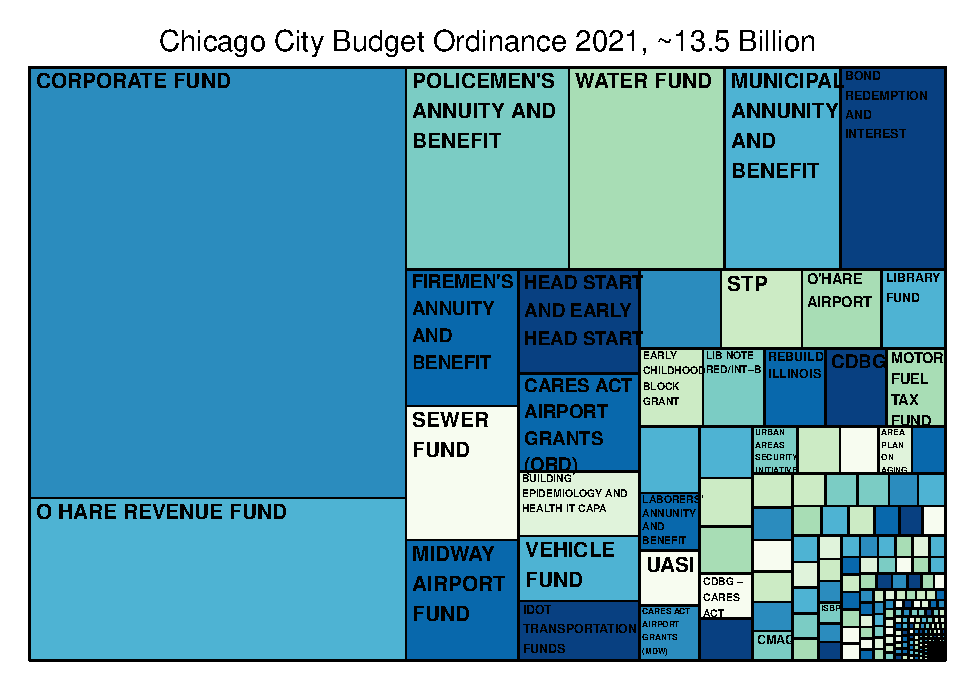
\includegraphics{cpd_budget_analysis_files/figure-latex/full budget treemap-1} \end{center}

The chart above gives us a superficial level of insight, but mostly
demonstrates the number of individual funds within the City budget; 251
in total. To aid legibility and increase information, I grouped all the
funds below the top ten largest into a `Miscellaneous' category. I also
shortened a few names and divided the appropriation amount by one
million so I could fit the dollar amount within the same square region.

\begin{center}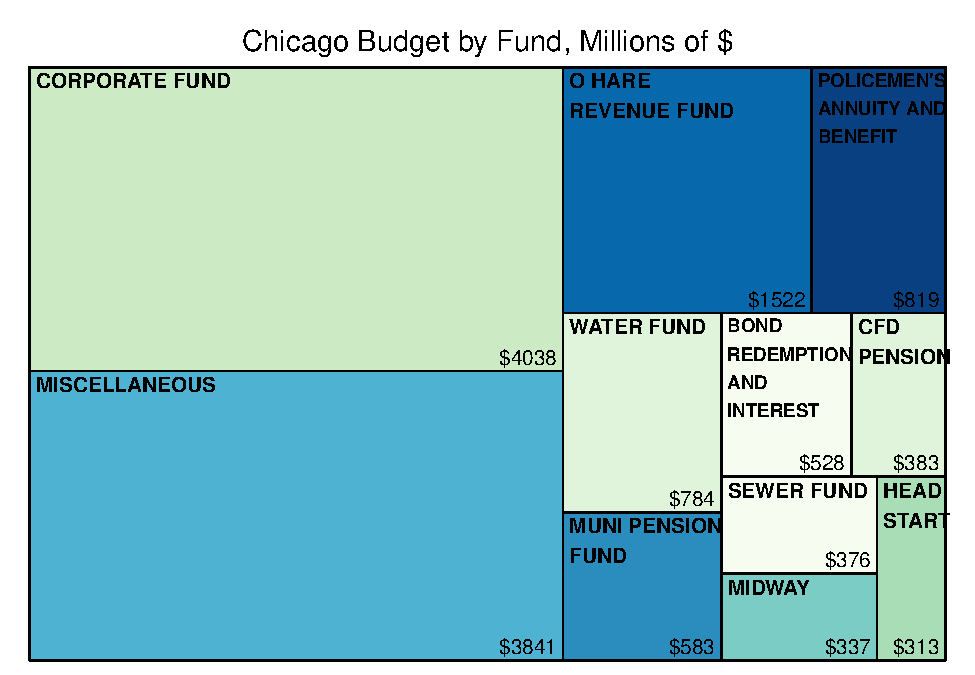
\includegraphics{cpd_budget_analysis_files/figure-latex/reduced budget treemap-1} \end{center}

In tabular format, we can include more exact numbers and add a
percentage column.

\begin{longtable}[]{@{}lcc@{}}
\caption{Chicago Budget Appropriations by Fund}\tabularnewline
\toprule
Fund Description & Total Appropriation (\$) & \% of Total\tabularnewline
\midrule
\endfirsthead
\toprule
Fund Description & Total Appropriation (\$) & \% of Total\tabularnewline
\midrule
\endhead
CORPORATE FUND & 4,037,639,000 & 29.86\tabularnewline
MISCELLANEOUS & 3,841,353,000 & 28.41\tabularnewline
O HARE REVENUE FUND & 1,521,857,000 & 11.25\tabularnewline
POLICEMEN'S ANNUITY AND BENEFIT & 818,850,000 & 6.06\tabularnewline
WATER FUND & 783,708,000 & 5.80\tabularnewline
MUNICIPAL ANNUNITY AND BENEFIT & 582,886,000 & 4.31\tabularnewline
BOND REDEMPTION AND INTEREST & 527,794,000 & 3.90\tabularnewline
FIREMEN'S ANNUITY AND BENEFIT & 382,779,000 & 2.83\tabularnewline
SEWER FUND & 375,696,000 & 2.78\tabularnewline
MIDWAY AIRPORT FUND & 336,559,000 & 2.49\tabularnewline
HEAD START AND EARLY HEAD START & 313,400,000 & 2.32\tabularnewline
\setlength{\parindent}{5ex} & &\tabularnewline
The Corporate Fund comprises about & 30\% of the total City budg & et at
\$4.03 billion. The proliferation of enterprise and special revenue
funds makes Miscellaneous the second biggest category. 33 different
departments get at least a portion of their budget from the Corporate
Fund, of which CPD is largest by a significant proportion at \$1.55
billion or 38.56\% of the total.\tabularnewline
\bottomrule
\end{longtable}

\begin{center}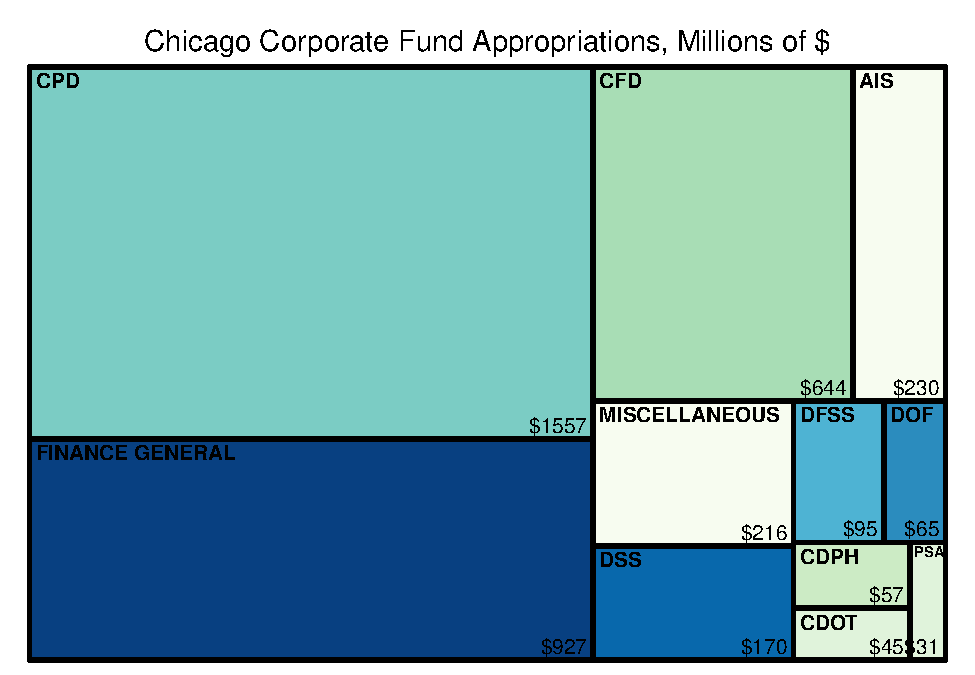
\includegraphics{cpd_budget_analysis_files/figure-latex/reduced corporate fund treemap-1} \end{center}

\begin{longtable}[]{@{}lcc@{}}
\caption{Corporate Fund by Department}\tabularnewline
\toprule
Dept Description & Total Appropriation (\$) & \% of Total\tabularnewline
\midrule
\endfirsthead
\toprule
Dept Description & Total Appropriation (\$) & \% of Total\tabularnewline
\midrule
\endhead
CPD & 1,556,831,274 & 38.56\tabularnewline
FINANCE GENERAL & 926,868,050 & 22.96\tabularnewline
CFD & 644,435,437 & 15.96\tabularnewline
AIS & 229,915,485 & 5.69\tabularnewline
MISCELLANEOUS & 215,991,727 & 5.35\tabularnewline
DSS & 170,125,492 & 4.21\tabularnewline
DFSS & 95,388,336 & 2.36\tabularnewline
DOF & 64,939,265 & 1.61\tabularnewline
CDPH & 57,344,506 & 1.42\tabularnewline
CDOT & 45,172,718 & 1.12\tabularnewline
PSA & 30,626,710 & 0.76\tabularnewline
\textbackslash setlength\{\parinde & nt\}\{5ex\} &\tabularnewline
Next, let's take a & quick look at Positions and & Salary data for the
City by department. One important note about the Positions and Salary
dataset is the `position control' variable that designates whether a
position is hourly or salaried. For our purposes, hourly positions need
to be filtered out because it affects how the position counts and
appropriations are counted. Salaried positions are counted individually,
and appropriations specify that annual salary for each position. Hourly
positions are counted in hours per position not number of positions, and
appropriations specify how much money is available to payout at the
hourly rate for a position. CPD hourly positions (mostly trainees)
account for roughly \$10 million.\tabularnewline
\bottomrule
\end{longtable}

\begin{longtable}[]{@{}lccrr@{}}
\caption{Positions by Department}\tabularnewline
\toprule
Department & Total Positions & \% of Positions & Salary App. (\$) & \%
Salary App.\tabularnewline
\midrule
\endfirsthead
\toprule
Department & Total Positions & \% of Positions & Salary App. (\$) & \%
Salary App.\tabularnewline
\midrule
\endhead
CPD & 14,051 & 42.22 & 1,261,135,566 & 42.10\tabularnewline
CFD & 5,124 & 15.40 & 544,271,849 & 18.17\tabularnewline
MISCELLANEOUS & 3,565 & 10.71 & 298,717,976 & 9.97\tabularnewline
DSS & 2,130 & 6.40 & 165,138,382 & 5.51\tabularnewline
CDA & 1,780 & 5.35 & 143,461,471 & 4.79\tabularnewline
DWM & 1,752 & 5.26 & 167,035,378 & 5.58\tabularnewline
CDOT & 1,181 & 3.55 & 111,329,366 & 3.72\tabularnewline
AIS & 1,125 & 3.38 & 106,006,661 & 3.54\tabularnewline
CPL & 913 & 2.74 & 65,690,560 & 2.19\tabularnewline
OEMC & 834 & 2.51 & 62,774,776 & 2.10\tabularnewline
CDPH & 828 & 2.49 & 69,715,524 & 2.33\tabularnewline
\bottomrule
\end{longtable}

The CPD employs 42\% of the City's total workforce and salary
appropriations. For a visual comparison of positions by department,
let's use a horizontal bar chart.

\begin{center}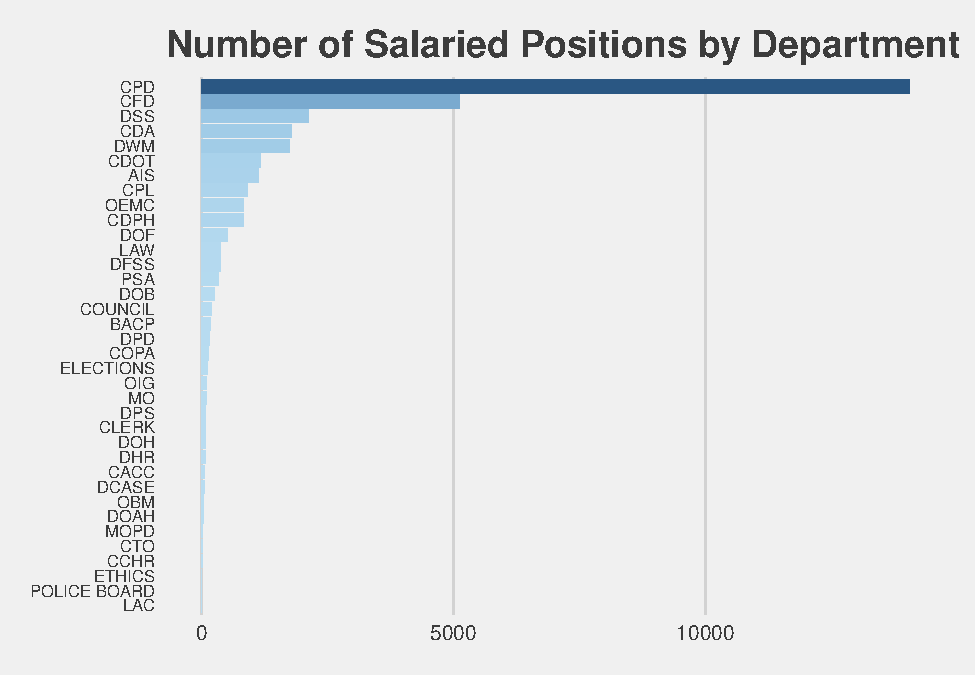
\includegraphics{cpd_budget_analysis_files/figure-latex/positions by dept bar chart-1} \end{center}

\hypertarget{cpd-budget-analysis}{%
\section{CPD Budget Analysis}\label{cpd-budget-analysis}}

\setlength{\parindent}{5ex}

The chart below shows a simplified list of the appropriations for the
CPD in the 2021 budget. For the sake of legibility, I filtered out any
items below \$2 million divided the amounts by \$1 million. CPD is
primarily a payroll expense, however, there are a few line items outside
of payroll that represent different forms of compensation. We'll explore
appropriation categories after a quick detour into the CPD Positions and
Salaries data.

\begin{center}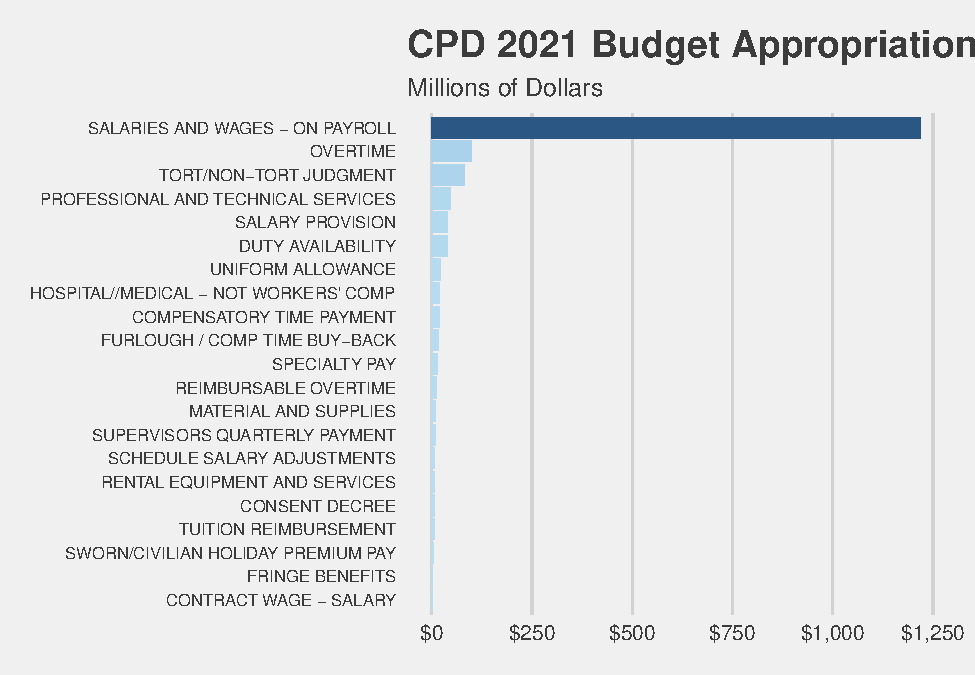
\includegraphics{cpd_budget_analysis_files/figure-latex/CPD appropriations by expense type-1} \end{center}

I decided to leave this particular table unreduced to fully display a
meaningful layer of complexity. There are 114 job titles within the CPD,
although many are different types of assignments for police officers.

\begin{longtable}[]{@{}lcc@{}}
\caption{CPD Appropriation by Job Title}\tabularnewline
\toprule
Title Description & Total Appropriation (\$) & Number of
Employees\tabularnewline
\midrule
\endfirsthead
\toprule
Title Description & Total Appropriation (\$) & Number of
Employees\tabularnewline
\midrule
\endhead
Police Officer & 816,484,008 & 9,693\tabularnewline
Sergeant & 157,590,024 & 1,316\tabularnewline
Police Officer - Assigned as Detective & 116,089,704 &
1,192\tabularnewline
Lieutenant & 37,198,824 & 271\tabularnewline
Police Officer - Assigned as Training Officer & 25,093,938 &
280\tabularnewline
Detention Aide & 15,677,904 & 229\tabularnewline
Police Officer - Assigned as Evidence Technician & 12,180,492 &
133\tabularnewline
Commander & 7,646,148 & 47\tabularnewline
Police Administrative Aide & 5,326,020 & 110\tabularnewline
Police Officer - Assigned as Explosives Detection Canine Handler &
5,237,946 & 59\tabularnewline
Captain & 4,200,072 & 28\tabularnewline
Senior Data Entry Operator & 4,185,036 & 63\tabularnewline
Police Officer - Assigned as Marine Officer & 3,168,360 &
34\tabularnewline
Police Officer - Assigned as Security Specialist & 2,387,562 &
22\tabularnewline
Deputy Chief & 2,381,568 & 14\tabularnewline
Police Officer - Assigned as Canine Handler & 2,365,092 &
26\tabularnewline
Police Officer - Assigned as Traffic Specialist & 2,156,562 &
24\tabularnewline
Police Officer - Assigned as Mounted Patrol Officer & 2,082,840 &
24\tabularnewline
Explosives Technician I & 2,070,834 & 19\tabularnewline
Community Organizer - CAPS & 1,790,388 & 24\tabularnewline
Criminal Intelligence Analyst & 1,748,976 & 21\tabularnewline
Clerk III & 1,631,196 & 27\tabularnewline
Police Technician & 1,617,636 & 17\tabularnewline
Training Officer & 1,600,560 & 17\tabularnewline
Property Custodian & 1,592,148 & 28\tabularnewline
Warrant and Extradition Aide & 1,476,528 & 21\tabularnewline
FOIA Officer & 1,438,596 & 24\tabularnewline
Principal Operations Analyst & 1,236,900 & 17\tabularnewline
Deputy Director & 1,234,584 & 9\tabularnewline
Fingerprint Technician II & 1,151,868 & 16\tabularnewline
Police Officer - Assigned as Latent Print Examiner & 1,038,588 &
13\tabularnewline
Assistant Director & 958,548 & 9\tabularnewline
Chief & 926,820 & 5\tabularnewline
Clinical Therapist III & 876,804 & 11\tabularnewline
Project Strategy Manager - CPD & 785,340 & 10\tabularnewline
Criminal History Analyst & 767,772 & 10\tabularnewline
Personal Computer Operator I & 682,416 & 11\tabularnewline
Administrative Assistant II & 583,428 & 8\tabularnewline
Police Forensic Investigator I & 567,042 & 5\tabularnewline
Subpoena Officer & 557,280 & 7\tabularnewline
Police Legal Officer II & 524,766 & 4\tabularnewline
Youth Services Coordinator & 470,712 & 6\tabularnewline
Police Officer Assigned as Helicopter Pilot & 453,768 & 5\tabularnewline
Fingerprint Technician III & 433,512 & 6\tabularnewline
Information Service Coordinator & 411,000 & 6\tabularnewline
Chief Performance Analyst & 371,712 & 4\tabularnewline
Paralegal II & 370,872 & 5\tabularnewline
Chief Operations Analyst & 368,712 & 4\tabularnewline
Clerk IV & 340,272 & 5\tabularnewline
Police Officer - Per Arbitration Award & 339,192 & 4\tabularnewline
Digital Intelligence Analyst & 323,520 & 5\tabularnewline
Research and Policy Analyst - CPD & 301,632 & 4\tabularnewline
Laboratory Technician & 291,816 & 4\tabularnewline
Senior Research Analyst & 275,832 & 3\tabularnewline
Accountant & 275,556 & 3\tabularnewline
Administrative Assistant III & 275,472 & 3\tabularnewline
Domestic Violence Advocate & 264,480 & 5\tabularnewline
Supervising Property Custodian & 263,784 & 4\tabularnewline
Superintendent of Police & 260,004 & 1\tabularnewline
Area Coordinator - CAPS & 249,468 & 3\tabularnewline
Associate Staff Attorney & 247,200 & 4\tabularnewline
Police Legal Officer I & 226,098 & 2\tabularnewline
Senior Performance Analyst & 215,688 & 3\tabularnewline
Information Coordinator & 210,816 & 3\tabularnewline
Staff Assistant & 201,432 & 2\tabularnewline
First Deputy Superintendent & 197,724 & 1\tabularnewline
Deputy Superintendent & 192,000 & 1\tabularnewline
Auditor III & 185,868 & 2\tabularnewline
Superintendent's Chief of Staff & 180,240 & 1\tabularnewline
Graphic Artist III & 168,072 & 2\tabularnewline
General Counsel & 165,516 & 1\tabularnewline
Attorney & 157,776 & 2\tabularnewline
Personnel Assistant & 149,076 & 2\tabularnewline
Public Relations Coordinator & 147,432 & 2\tabularnewline
Crime Victim Advocate & 146,880 & 3\tabularnewline
Fingerprint Technician IV & 139,776 & 2\tabularnewline
Director of Professional Counseling Services & 138,348 &
1\tabularnewline
Director of News Affairs & 135,672 & 1\tabularnewline
Director of CAPS & 134,292 & 1\tabularnewline
Personal Computer Operator II & 132,816 & 2\tabularnewline
Assistant General Counsel & 126,504 & 1\tabularnewline
Director of Police Records & 121,260 & 1\tabularnewline
Senior Programmer/Analyst & 119,712 & 1\tabularnewline
Director of Research and Planning & 119,148 & 1\tabularnewline
Public Information Officer & 116,040 & 2\tabularnewline
Assistant Director of News Affairs & 115,656 & 1\tabularnewline
Risk Manager-CPD & 115,656 & 1\tabularnewline
Program Analyst & 110,508 & 1\tabularnewline
Criminalist III & 109,620 & 1\tabularnewline
Forensic Firearm / Toolmark Examiner & 108,960 & 1\tabularnewline
Coordinator of Special Projects & 105,420 & 1\tabularnewline
Firearms Identification Technician I & 104,502 & 1\tabularnewline
Police Officer - Assigned as Supervising Latent Print Examiner & 104,502
& 1\tabularnewline
Police Officer - Assigned as Supervising Substance Abuse Counselor &
104,502 & 1\tabularnewline
Director of Administration II & 100,668 & 1\tabularnewline
Police Agent & 98,052 & 1\tabularnewline
Assistant to the Executive Director & 96,096 & 1\tabularnewline
Coordinator of Community Services & 87,564 & 1\tabularnewline
Personal Computer Operator III & 76,248 & 1\tabularnewline
Projects Administrator & 75,408 & 1\tabularnewline
Auditor II & 71,196 & 1\tabularnewline
Senior Intelligence Analyst & 70,272 & 1\tabularnewline
Compliance Officer & 70,140 & 1\tabularnewline
Language Access Coordinator & 70,140 & 1\tabularnewline
Programmer/Analyst & 69,048 & 1\tabularnewline
Police Officer - Assigned as Armorer & 68,616 & 1\tabularnewline
Principal Storekeeper & 66,336 & 1\tabularnewline
Senior Labor Relations Specialist & 64,320 & 1\tabularnewline
Community Outreach Coordinator & 63,720 & 1\tabularnewline
Payment Services Representative & 60,420 & 1\tabularnewline
Executive Administrative Assistant II & 58,968 & 1\tabularnewline
Assistant Supervisor of Police Records & 53,736 & 1\tabularnewline
Manager of Data Entry Operators & 53,736 & 1\tabularnewline
Photographic Specialist & 53,736 & 1\tabularnewline
\setlength{\parindent}{5ex} & &\tabularnewline
The primary distinction between CPD job titles is between peace offic &
ers and non-peace officers & as defined by under Illinois statute (720
ILCS 5/2-13 \footnote{\url{https://www.ilga.gov/legislation/ilcs/fulltext.asp?DocName=072000050K2-13}}).
The Office of the Inspector General (OIG) maintains a list of job title
codes that signify peace officer designation \footnote{\url{https://informationportal.igchicago.org/cpd-sworn-officer-unit-assignments/}}.
I used this list of job title codes as a reference applied to job title
codes in the Positions and Salaries dataset to divide CPD employees into
either category. However, several police officer assignments and the
Deputy Superintendent were not included in the OIG list. Using basic
knowledge and inductive reasoning, I applied the peace officer
designation to all relevant job title codes and
descriptions.\tabularnewline
\bottomrule
\end{longtable}

\begin{center}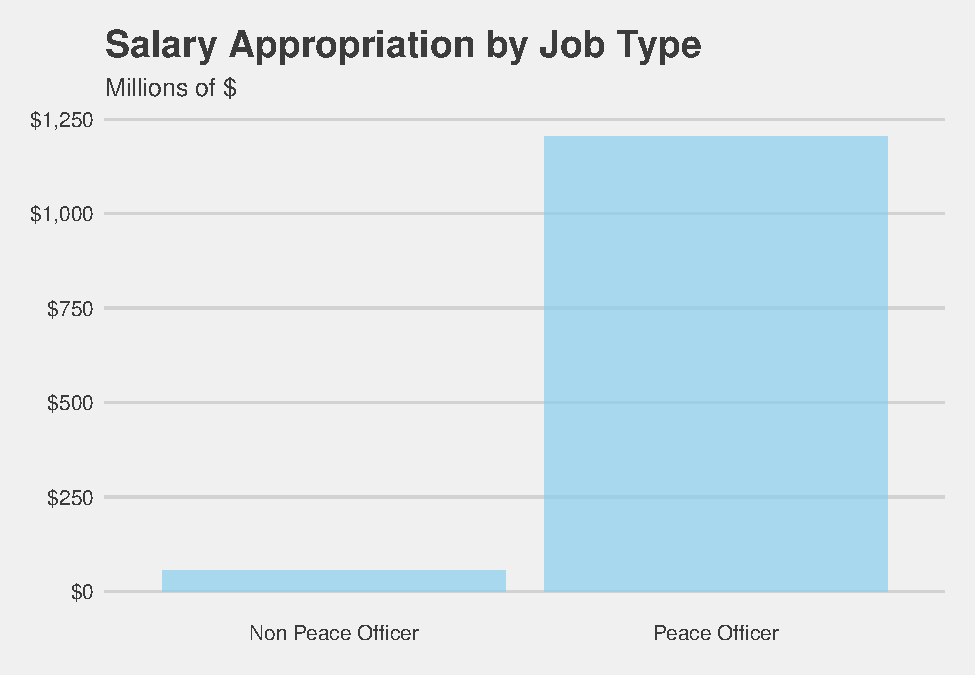
\includegraphics{cpd_budget_analysis_files/figure-latex/appropriation by PO status-1} \end{center}

Although the budget appropriation for peace officer salaries is much
higher than non-peace officers, their average annual salary ranges are
fairly close. This is the broadest categorization possible, so future
research could reveal more about how the hierarchy among peace officers
affects compensation costs.

\begin{center}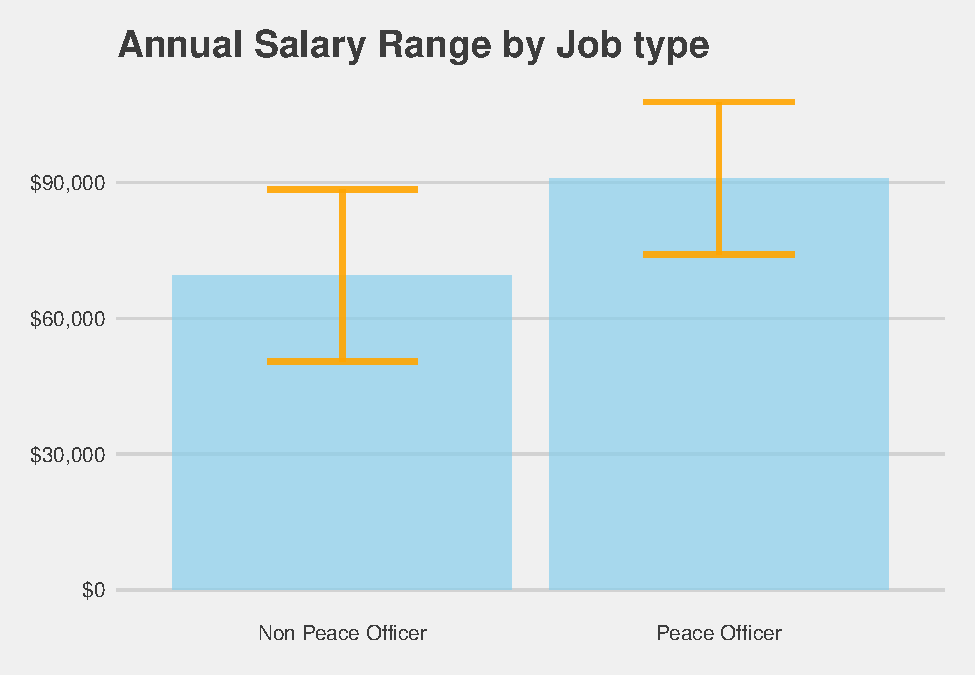
\includegraphics{cpd_budget_analysis_files/figure-latex/PO vs. non-PO salary range-1} \end{center}

\hypertarget{total-policing-costs}{%
\section{Total Policing Costs}\label{total-policing-costs}}

\setlength{\parindent}{5ex}

The price of police is more than the CPD budget line in the City
government. Most notably, the Policemen's Annuity and Benefit Fund
(pension) is an actuarial fund completely separate from the Corporate
Fund that falls under the authority of the City Department on Finance.
State law mandates the level of yearly City contributions to the pension
fund, which are set to increase until the fund reaches actuarial
solvency. Other meaningful costs is the Civilian Office of Police
Accountability, the Police Board, and various Consent Decree \footnote{\url{http://chicagopoliceconsentdecree.org/}}
appropriations scattered across different departments. Below is a table
of all the appropriations either contained within the CPD budget
specifically or ancillary to it. This list is almost certainly not
exhaustive, but based on what I can surmise for myself, the grand total
for policing in Chicago for Fiscal Year 2021 is \$2.53 billion.

\begin{longtable}[]{@{}lc@{}}
\caption{Total Costs}\tabularnewline
\toprule
Appropriation Type & Total Appropriation (\$)\tabularnewline
\midrule
\endfirsthead
\toprule
Appropriation Type & Total Appropriation (\$)\tabularnewline
\midrule
\endhead
SALARIES AND WAGES - ON PAYROLL & 1,230,229,131\tabularnewline
EMPLOYEE ANNUITY AND BENEFIT & 786,793,000\tabularnewline
OVERTIME & 99,641,798\tabularnewline
TORT/NON-TORT JUDGMENT & 82,558,000\tabularnewline
PROFESSIONAL AND TECHNICAL SERVICES & 47,291,956\tabularnewline
SALARY PROVISION & 40,023,092\tabularnewline
DUTY AVAILABILITY & 39,525,800\tabularnewline
LOSS IN COLLECTION OF TAXES & 32,057,000\tabularnewline
UNIFORM ALLOWANCE & 22,273,775\tabularnewline
HOSPITAL//MEDICAL - NOT WORKERS' COMP & 19,243,000\tabularnewline
COMPENSATORY TIME PAYMENT & 18,569,385\tabularnewline
FURLOUGH / COMP TIME BUY-BACK & 15,923,324\tabularnewline
SPECIALTY PAY & 14,905,625\tabularnewline
REIMBURSABLE OVERTIME & 12,700,000\tabularnewline
CONSENT DECREE & 9,956,491\tabularnewline
MATERIAL AND SUPPLIES & 9,618,655\tabularnewline
SUPERVISORS QUARTERLY PAYMENT & 9,447,500\tabularnewline
RENTAL EQUIPMENT AND SERVICES & 8,385,100\tabularnewline
SCHEDULE SALARY ADJUSTMENTS & 8,068,749\tabularnewline
TUITION REIMBURSEMENT & 7,340,000\tabularnewline
SWORN/CIVILIAN HOLIDAY PREMIUM PAY & 4,123,484\tabularnewline
FRINGE BENEFITS & 3,148,943\tabularnewline
CONTRACT WAGE - SALARY & 2,992,515\tabularnewline
DELEGATE AGENCIES & 1,823,000\tabularnewline
INDIRECT COSTS & 828,454\tabularnewline
RENTAL-DATA HARDWARE EQ & 787,461\tabularnewline
SOFTWARE MAINTENANCE AND LICENSING & 700,369\tabularnewline
REPAIR PARTS AND MATERIAL & 497,718\tabularnewline
PAYMENT RETROACTIVE SALARIES & 438,052\tabularnewline
MACHINERY AND EQUIPMENT & 389,000\tabularnewline
TECHNICAL MEETING COSTS & 360,238\tabularnewline
REPAIR/MAINT EQUIPMENT & 304,822\tabularnewline
REIMBURSEMENT - DSS & 250,000\tabularnewline
FOOD & 237,250\tabularnewline
VEHICLES & 125,000\tabularnewline
STIPENDS & 111,000\tabularnewline
VIOLENCE REDUCTION PROGRAM & 100,000\tabularnewline
TRANSPORTATION AND EXPENSE ALLOWANCE & 98,500\tabularnewline
COURT REPORTING & 85,000\tabularnewline
DUES SUBSC \& MEM & 73,699\tabularnewline
MOBILE COMMUNICATION SERVICES & 70,017\tabularnewline
TECHNICAL AND SCIENTIFIC EQUIPMENT & 66,000\tabularnewline
LIVESTOCK & 54,600\tabularnewline
WASTE DISPOSAL SERVICES & 40,710\tabularnewline
LEASE/PURCHASE EQUIPMENT & 29,500\tabularnewline
CLOTHING & 29,175\tabularnewline
TELEPHONE - CENTREX BILLINGS & 21,000\tabularnewline
APPARATUS AND INSTRUMENTS & 18,658\tabularnewline
BOOKS AND RELATED MATERIAL & 18,471\tabularnewline
OUTSIDE GRAPHIC SERVICES & 17,500\tabularnewline
STATIONERY AND OFFICE SUPPLIES & 16,125\tabularnewline
CULTURAL PROGRAMMING GRANTS & 12,000\tabularnewline
DRUGS MEDICINE AND CHEMICAL MATERIALS & 10,041\tabularnewline
FREIGHT AND EXPRESS CHARGES & 10,000\tabularnewline
POSTAGE & 6,000\tabularnewline
REIMBURSEMENT - AIS & 5,000\tabularnewline
ADVERTISING & 2,400\tabularnewline
GRAPHIC DESIGN SERV & 1,500\tabularnewline
LOCAL TRANSPORTATION & 1,500\tabularnewline
IT MAINTENANCE & 1,000\tabularnewline
LICENSE STICKER TAG AND PLATES & 750\tabularnewline
GASOLINE & 500\tabularnewline
CLEANING AND SANITATION SUPPLIES & 381\tabularnewline
OFFICE AND BUILDING SERVICES & 300\tabularnewline
TELEPHONE - MAINTENANCE & 300\tabularnewline
\bottomrule
\end{longtable}

To simplify this table, I created four categories for medical costs,
non-salary compensation, physical assets, and professional services.

\begin{center}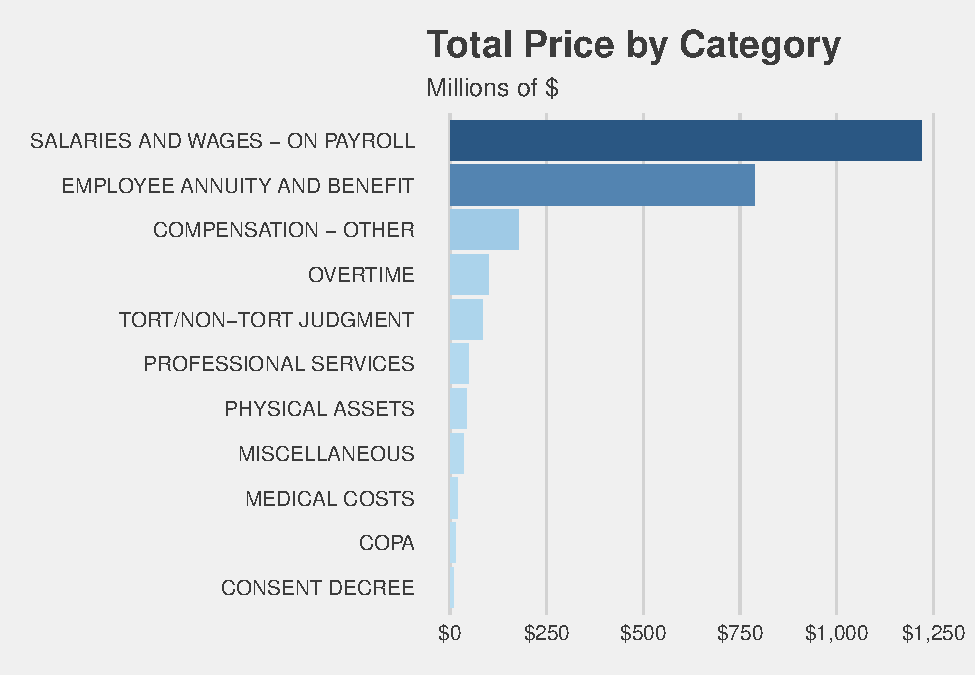
\includegraphics{cpd_budget_analysis_files/figure-latex/total price by category reduced-1} \end{center}

\hypertarget{conclusion}{%
\section{Conclusion}\label{conclusion}}

\setlength{\parindent}{5ex}

The total Chicago Police Department Budget Appropriation (including
appropriations outside the Corporate Fund) is \$1.6 billion dollars for
Fiscal Year 2021, or 12.56\% of the full City budget. It's proportion of
the Corporate Fund is \$1.5 billion or 38.56\%. Most City employees work
for the CPD (\textasciitilde14 thousand) and the overwhelming majority
of salary expenses flow towards that department. However, the budget
line for CPD does not capture all the direct costs of policing for the
City. Pension contributions (\$818 million), the Civilian Office of
Police Accountability, the Police Board, and various Consent Decree
expenses bring the total up to \$2.5 billion.
\setlength{\parindent}{5ex} Opportunities for future research include a
closer look at personnel costs and how compensation is structured
through the CPD hierarchy. The City also maintains datasets on crime and
COPA cases, which could prove insightful with regard to effectiveness
and performance measures. These data along with past City budgets can
shed light on what has come before, where we are now, and what the
future may hold. There is also a vast literature that can enhance my
qualitative analysis that I am eager to reengage.

\end{document}
